\section{DETESTS-Dis}

\begin{frame}{Descripción de la tarea}
    \begin{columns}
        \column{0.5\textwidth}
            \begin{itemize}
                \item Segunda edición de DETESTS. Enmarcada dentro de LeWiDi.
                \item Dos tareas:
                    \begin{itemize}
                        \item \textbf{Detección de estereotipos}
                        \item \textbf{Categorización de estereotipos} en explícitos o implícitos 
                    \end{itemize}
                \item Dataset:
            \begin{itemize}
                \item Hilos de conversaciones (X y foros de noticias)
                \item Contexto proporcionado
                \item Etiquetas agregadas y sin agregar
                \item 3 anotadores (2 lingüistas y 1 investigador)
            \end{itemize}
    \end{itemize}
        \column{0.5\textwidth}
        \centering
        \includesvg[width=0.8\textwidth]{images/DETESTS-tareas.svg}
        % Please add the following required packages to your document preamble:
        % \usepackage{graphicx}
        \begin{table}[]
            \small
            \centering
            \resizebox{\textwidth}{!}{%
            \begin{tabular}{|p{3.5cm}|c|c|}
            \hline
            Texto                                                                                                                                                     & Estereotipo & Implícito  \\ \hline
            La solución es desarrollar el pensamiento crítico y escéptico.                                                                                            & X           & -          \\ \hline
            Guste o no guste la cosa está clara: si no hubiera moros en Europa esto no pasaría.                           & \checkmark  & X          \\ \hline
            Ayer estuve en hacienda tributando, todos españoles, por la tarde fui al centro de salud, españoles, la mitad. & \checkmark  & \checkmark \\ \hline
            \end{tabular}%
            }
            
            %\caption{}
            %\label{tab:my-table}
            \end{table}
    \end{columns}
\end{frame}

\begin{frame}{Análisis de los datos}
    \begin{columns}[T]
        \column{0.5\textwidth}
        \centering
        Identificación de estereotipos
        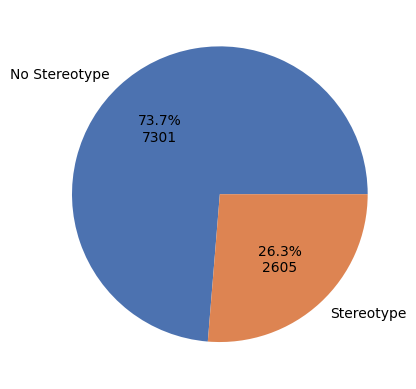
\includegraphics[width=\textwidth]{images/detest_hard_labels.png}

        \column{0.5\textwidth}
        Categorización de estereotipos
        \centering
        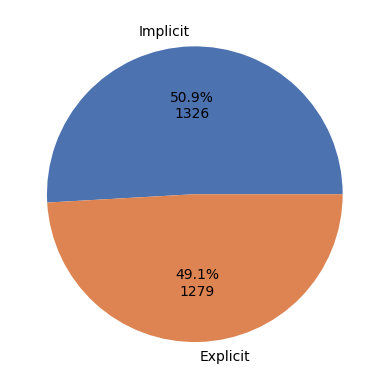
\includegraphics[width=\textwidth]{images/detest_soft_labels.png}
    \end{columns}

\end{frame}

\begin{frame}{Propuesta de sistema}
    \begin{columns}
    \column{0.6\textwidth}
    \begin{itemize}
        \item RoBERTa model as encoder. Our appro
        \item 
        \item Tres arquitecturas distintas
            \begin{itemize}
                \item \textit{Hard label}: Train by hard label, no disagreements considered
                \item \textit{Soft label approach}
                \item \textit{Multi-task}: Predecir cada anotación individualmente
            \end{itemize}

        \item \textit{Layer-Wise Learning Rate fine-tuning}
        \begin{itemize}
            \item Deeper layers are updated more aggresively than shallower layers
            \item $\eta = \{1e-5, 2e-5, 5e-5, 1e-4\}$
            \item $\xi = \{1'0, 0'97, 0'95, 0'90\}$
        \end{itemize}
        \item \textit{Back translation}
        \item Inclusión de Contexto
    \end{itemize}
    
    \column{0.4\textwidth}
    \centering
    \includesvg[width=4.5cm]{images/DETESTS-dis_presentacion.svg}
    \end{columns}
\end{frame}

\begin{frame}{Resultados detección de estereotipos}

\begin{table}[hbt]
\centering
\resizebox{\textwidth}{!}{%
\begin{tabular}{c|cc||cc|}
\cline{2-5}
                                          & \multicolumn{2}{c||}{Hard evaluation}                       & \multicolumn{2}{c|}{Soft evaluation}                                      \\ \hline
\multicolumn{1}{|c|}{Arquitectura}        & \multicolumn{1}{c|}{\# ranking/21} & F1 Score $\uparrow$ & \multicolumn{1}{c|}{\# ranking/8} & \textit{Cross Entropy} $\downarrow$ \\ \hline
\multicolumn{1}{|c|}{\textit{Hard label}} & \multicolumn{1}{c|}{7}               & 0.653               & \multicolumn{1}{c|}{8}              & 1.409                               \\ \hline
\multicolumn{1}{|c|}{\textit{Soft label}} & \multicolumn{1}{c|}{\textbf{4}}      & \textbf{0.691}      & \multicolumn{1}{c|}{\textbf{2}}     & \textbf{0.850}                      \\ \hline
\multicolumn{1}{|c|}{\textit{Multi-task}} & \multicolumn{1}{c|}{5}               & 0.685               & \multicolumn{1}{c|}{7}              & 1.081                               \\ \hline \hline
\multicolumn{1}{|c|}{Gold baseline}       & \multicolumn{1}{c|}{0}               & 1.000               & \multicolumn{1}{c|}{0}              & 0.255                               \\ \hline
\multicolumn{1}{|c|}{Ganadores}           & \multicolumn{1}{c|}{1}               & 0.720               & \multicolumn{1}{c|}{1}              & 0.841                               \\ \hline
\multicolumn{1}{|c|}{Baseline BETO}       & \multicolumn{1}{c|}{6}               & 0.663               & \multicolumn{1}{c|}{4}              & 0.893                               \\ \hline
\end{tabular}%
}
\caption{Resultados obtenidos en la tarea de identificación de estereotipos de DETESTS-Dis. En negrita, nuestros mejores resultados.}
\label{tab:t1_detests}
\end{table}
\footfullcite{detests_dis_2024}
\end{frame}

\begin{frame}{Resultados categorización de estereotipos}

% Please add the following required packages to your document preamble:
% \usepackage{graphicx}
\begin{table}[]
\centering
\resizebox{\textwidth}{!}{%
\begin{tabular}{c|ccc||ccc|}
\cline{2-7}
                                          & \multicolumn{3}{c||}{Hard evaluation}                                                             & \multicolumn{3}{c|}{Soft evaluation}                                                                      \\ \hline
\multicolumn{1}{|c|}{Arquitectura}        & \multicolumn{1}{c|}{\# ranking/14} & \multicolumn{1}{c|}{ICM $\uparrow$} & ICM Norm $\uparrow$ & \multicolumn{1}{c|}{\# ranking/6} & \multicolumn{1}{c|}{ICM Soft $\uparrow$} & ICM Soft Norm $\uparrow$ \\ \hline
\multicolumn{1}{|c|}{\textit{Hard label}} & \multicolumn{1}{c|}{4}               & \multicolumn{1}{c|}{0.045}          & 0.516               & \multicolumn{1}{c|}{2}              & \multicolumn{1}{c|}{-0.917}              & 0.401                    \\ \hline
\multicolumn{1}{|c|}{\textit{Soft label}} & \multicolumn{1}{c|}{\textbf{2}}      & \multicolumn{1}{c|}{\textbf{0.065}} & \textbf{0.524}      & \multicolumn{1}{c|}{3}              & \multicolumn{1}{c|}{-0.969}              & 0.396                    \\ \hline
\multicolumn{1}{|c|}{\textit{Multi-task}} & \multicolumn{1}{c|}{3}               & \multicolumn{1}{c|}{0.061}          & 0.522               & \multicolumn{1}{c|}{\textbf{1}}     & \multicolumn{1}{c|}{\textbf{-0.900}}     & \textbf{0.403}           \\ \hline \hline
\multicolumn{1}{|c|}{Gold baseline}       & \multicolumn{1}{c|}{0}               & \multicolumn{1}{c|}{1.380}          & 1.000               & \multicolumn{1}{c|}{0}              & \multicolumn{1}{c|}{4.651}               & 1.000                    \\ \hline
\multicolumn{1}{|c|}{Baseline BETO}       & \multicolumn{1}{c|}{1}               & \multicolumn{1}{c|}{0.126}          & 0.546               & \multicolumn{1}{c|}{4}              & \multicolumn{1}{c|}{-1.124}              & 0.379                    \\ \hline
\end{tabular}%
}
\caption{Resultados obtenidos en la tarea de categorización de estereotipos de DETESTS-Dis. En negrita, nuestros mejores resultados.}
\label{tab:t2_detests}
\end{table}
\footfullcite{detests_dis_2024}

\end{frame}